\documentclass[a4paper,12pt,headsepline]{scrartcl}

%\part{title}
\usepackage[utf8]{inputenc}
\usepackage{graphicx}
\usepackage{caption,subcaption}
\usepackage[british]{babel}
\usepackage[T1]{fontenc}
\usepackage{geometry}
\usepackage{proof}
\geometry{left=3.5cm, right=2cm, top=2.5cm, bottom=2cm}
\usepackage{hyperref}
%\usepackage[hyphens,obeyspaces,spaces]{url}
\usepackage{fancybox}
\usepackage{amssymb,amsmath,amsthm}
\usepackage{gensymb}
\usepackage[linesnumbered,ruled,vlined,norelsize]{algorithm2e}
%\usepackage[bookmarksnumbered,pdftitle={\titleDocument},hyperfootnotes=false]{hyperref} 
\usepackage{color}
\usepackage{float}
\usepackage{enumerate}
\usepackage{marvosym}
\usepackage{tikz}
\usetikzlibrary{positioning}
\usetikzlibrary{patterns}
\usepackage{tikz-network}
\usepackage{pgfplots}
\pgfplotsset{compat=1.12}
\usepgfplotslibrary{fillbetween}
%%%

% Always forgetting the figure parameters for precise graphical inclusions -.-

%\begin{figure}[H]
	%\centering
	%\begin{subfigure}{0.4\textwidth}
		%\centering
		%\includegraphics[width=0.34\linewidth,page=6]{includegraphics/L-%t-shape_candidates}
%		\caption{Empty $T$-face}\label{im:empty_T}	
%	\end{subfigure}
%%%
%test
%\usepackage[backend=bibtex]{biblatex}
%\usepackage{filecontents}

%\addbibresource{ref.bib}

\restylefloat{figure}

% Makros
%\newenvironment{sketch}{\begin{proof}[Proof (Sketch)]}{\end{proof}}
%\newtheorem{theorem}{Theorem}
%\newtheorem{assumption}{Assumption}
\newtheorem{lemma}{Lemma}
%\newtheorem{remark}{Remark}
%\newtheorem{definition}{Definition}
%\newtheorem{corollary}{Corollary}
\newcommand{\comment}[1]
{
  \begin{quotation}
    \textcolor{blue}{\underline{Edit:} #1}
  \end{quotation}
}
\newtheorem{aufgabe}{Exercise}
\newcommand{\Ex}[2]
{
	\setcounter{section}{#2}
	\section*{Übungsblatt #2 zu #1}
}
\newcommand{\TODO}[1]
{
  \begin{quotation}
    \textcolor{red}{\underline{TODO:} #1}
  \end{quotation}
}
% Zeichen 
\newcommand{\OO}{\ensuremath{\mathcal{O}}}
\newcommand{\ec}{\texttt{ec}}
\newcommand{\NP}{\call{NP}}
\newcommand{\call}[1]{\ensuremath{\mathcal{#1}}}

% neue Kopfzeilen mit fancypaket
\usepackage{fancyhdr} %Paket laden
\pagestyle{fancy} %eigener Seitenstil
\fancyhf{} %alle Kopf- und Fußzeilenfelder bereinigen
\fancyhead[L]{Benjamin \c Coban \\ Christoph Jabs}
\fancyhead[C]{Algorithmen und Komplexität \\ Blatt 8}
\fancyhead[R]{3526251 \\ 5567177}
\setlength{\headheight}{39pt}
\renewcommand{\headrulewidth}{0.4pt} %obere Trennlinie
%\fancyfoot[C]{\thepage} %Seitennummer
%\renewcommand{\footrulewidth}{0.4pt} %untere Trennlinie

\frenchspacing
\makeindex

% Pseudocode für Java
\usepackage{listings}
\lstset{numbers=left, numberstyle=\tiny, numbersep=5pt, keywordstyle=\color{black}\bfseries, stringstyle=\ttfamily,showstringspaces=false,basicstyle=\footnotesize,captionpos=b}
\lstset{language=java}

% Disable single lines at the start of a paragraph (Schusterjungen)
\clubpenalty = 10000
% Disable single lines at the end of a paragraph (Hurenkinder)

\widowpenalty = 10000
\displaywidowpenalty = 10000
\begin{document}
\begin{aufgabe}ILP
\end{aufgabe}
\begin{enumerate}[a)]
	\item ILP with enumerated vertices:
    \begin{alignat*}{3}
      \textbf{\text{maximize}}\quad && \sum x_i \\
      \textbf{\text{s.t.}}\quad     && x_i + x_j &\leq 1 &&\quad\forall (i,j)\in E\\
                                    && x_i &\in \{0,1\}  &&\quad\forall i \in V
    \end{alignat*}
  \item By removing one or more of the constraints of a linear program, the feasible set is increased to a superset of the original feasible region.
    All of the points that were originally feasible are therefore still in the new feasible region.
    That the solution to the relaxed linear program must be at least as large can be shown with a simple contradiction:
    If the solution to the relaxed problem was smaller than the solution to the original problem, than the feasible region to the relaxed problem does still contain the optimal solution to the original problem, which yields a higher objective value than the solution found to the relaxed problem.
    Therefore the solution to the original problem is a better solution to the relaxed problem and the solution with a smaller value cannot be optimal.
  \item Consider a fully connected graph with three vertices:
    \[ K_3 = (\{u_1,u_2,u_3\},\{(u_1,u_2),(u_2,u_3),(u_3,u_1)\}) \]
    The maximum independent set for this graph does only contain one of the vertices (e.g. $x=(0,0,1)^T$), therefore the objective value of the ILP is 1.
    However, if we consider the relaxed version of the linear program, we can assign a value of 0.5 to each of the vertices ($x=(0.5,0.5,0.5)^T$).
    This solution does still satisfy all the constraints and the corresponding objective value is 1.5.
\end{enumerate}
\newpage
\begin{aufgabe}Planar graph properties
\end{aufgabe}
Following Eulers Theorem:
\begin{align*}
n + f = m + 2
\end{align*}
A maximal planar graph has exactly $3n-6$ edges, meaning:
\begin{align*}
n + f = 3n-6 + 2   \Rightarrow f = 2n-4
\end{align*}
\begin{enumerate}[a)]
	\item It is to proof that for a planar embedded graph $G$ with $n$ vertices and $m$ edges without any triangles the following holds:
	\begin{align*}
		m \leq 2n-4
	\end{align*}
	\begin{proof}
		Consider a maximal planar graph $G'$ with $n$ vertices. Then, it holds that $G'$ has exactly $m' = 3n-6$ edges and $f' = 2n-4$ faces. Since $G'$ is maximal planar, every face is a triangle. A planar graph $G$ without any triangles can be constructed by removing an edge between two adjacent faces. Then, two triangles become one quadrangle. Since $G'$ has exactly $2n-4$ edges, there are $n-2$ edge removals to obtain a planar graph without any triangles. Therefore $G$ can hold at most $m \leq m' - (n-2) = 2n -4$ edges.
	\end{proof}
	\item It is to examine what an upper bound of edge counts might be when a planar embedded graph $G'$ ain't got any cycles of size three or four. The following holds:
	\begin{align*}
		m \leq \frac{5}{3}n - \frac{10}{3}
	\end{align*}
	\begin{proof}
		Again, a maximal planar graph $G'$ with $n$ vertices holds exactly $m' = 3n-6$ edges and $f' = 2n-4$ faces. From $G'$, the removal of two neighbouring edges of three adjacent triangles will result in a residual graph $G$ with cycles of size at least 5. So, in count, for every three triangles two edges will be removed. Therefore it holds, that $m \leq m' - \frac{2\cdot (2n-4)}{3} = 3n-6 - (\frac{4}{3}n - \frac{8}{3}) = \frac{5}{3}n - \frac{10}{3}$.
	\end{proof}
\end{enumerate}
\newpage
\begin{aufgabe}Planarity
\end{aufgabe}
\begin{enumerate}[a)]
  \item The given graph has $n=9$ vertices and $m=24$ edges.
    From the lecture we know that for a planar graph, $m\le3n-6$ must hold and therefore a graph that does not satisfy this condition cannot be planar.
    For $n=9$ and $m=24$, this condition does not hold, therefore this graph is not planar.
  \item We will show that this graph is planar by drawing it as a drawing with no crossing edges.
    To be able to recognise the vertices and edges more easily, we first mark the ones that will be moved in orange:
    \begin{center}
      \begin{tikzpicture}
        \Vertex[size=.3]{A}
        \Vertex[size=.3,x=1.2,y=-1]{B}
        \Vertex[size=.3,x=-1.2,y=-1,color=orange]{C}
        \Vertex[size=.3,x=-.8,y=-2]{D}
        \Vertex[size=.3,x=.8,y=-2]{E}
        \Vertex[size=.3,x=1.2,y=1]{F}
        \Vertex[size=.3,x=2,y=0,color=orange]{G}
        \Vertex[size=.3,x=2.2,y=-1,color=orange]{H}
        \Vertex[size=.3,x=2.2,y=-2]{I}

        \Edge(A)(B)
        \Edge(A)(C)
        \Edge(B)(E)
        \Edge(C)(D)
        \Edge(E)(D)
        \Edge(A)(F)
        \Edge(F)(G)
        \Edge(G)(B)
        \Edge(B)(F)
        \Edge(A)(G)
        \Edge(B)(H)
        \Edge(H)(I)
        \Edge(I)(E)
        \Edge(E)(H)
        \Edge(B)(I)
        \Edge(C)(B)
        \Edge(C)(E)
        \Edge[color=orange](D)(B)
        \Edge(A)(D)
      \end{tikzpicture}
    \end{center}
    Now we move the marken vertices and edges and therefore get a planar drawing:
    \begin{center}
      \begin{tikzpicture}
        \Vertex[size=.3]{A}
        \Vertex[size=.3,x=1.2,y=-1]{B}
        \Vertex[size=.3,y=-1,color=orange]{C}
        \Vertex[size=.3,x=-.8,y=-2]{D}
        \Vertex[size=.3,x=.8,y=-2]{E}
        \Vertex[size=.3,x=1.2,y=1]{F}
        \Vertex[size=.3,x=.8,y=0,color=orange]{G}
        \Vertex[size=.3,x=1.4,y=-1.7,color=orange]{H}
        \Vertex[size=.3,x=2.2,y=-2]{I}

        \Edge(A)(B)
        \Edge(A)(C)
        \Edge(B)(E)
        \Edge(C)(D)
        \Edge(E)(D)
        \Edge(A)(F)
        \Edge(F)(G)
        \Edge(G)(B)
        \Edge(B)(F)
        \Edge(A)(G)
        \Edge(B)(H)
        \Edge(H)(I)
        \Edge(I)(E)
        \Edge(E)(H)
        \Edge(B)(I)
        \Edge(C)(B)
        \Edge(C)(E)
        \Edge[path={D,{2.5,-2.5},{2.5,-1},B},color=orange](D)(B)
        \Edge(A)(D)
      \end{tikzpicture}
    \end{center}
  \item To show that this graph is not planar, we show that it contains a subdivision of $K_5$.
    Consider the subgraph marked in orange.
    \begin{center}
      \begin{tikzpicture}
        \Vertex[size=.3,color=orange]{A}
        \Vertex[size=.3,x=1.2,y=-1,color=orange]{B}
        \Vertex[size=.3,x=-1.2,y=-1,color=orange]{C}
        \Vertex[size=.3,x=-.8,y=-2,color=orange]{D}
        \Vertex[size=.3,x=.8,y=-2,color=orange]{E}
        \Vertex[size=.3,x=1.2,y=1]{F}
        \Vertex[size=.3,x=2,y=-.5,color=orange]{G}
        \Vertex[size=.3,x=2.2,y=-2]{I}

        \Edge[color=orange](A)(B)
        \Edge[color=orange](A)(C)
        \Edge[color=orange](B)(E)
        \Edge[color=orange](C)(D)
        \Edge[color=orange](E)(D)
        \Edge(A)(F)
        \Edge(F)(G)
        \Edge(G)(B)
        \Edge(B)(F)
        \Edge[color=orange](A)(G)
        \Edge(B)(G)
        \Edge(G)(I)
        \Edge(I)(E)
        \Edge[color=orange](E)(G)
        \Edge(B)(I)
        \Edge[color=orange](C)(B)
        \Edge[color=orange](C)(E)
        \Edge[color=orange](D)(B)
        \Edge[color=orange](A)(D)
      \end{tikzpicture}
    \end{center}
    We can redraw this and see that this as follows and see that this is a subdivision of $K_5$ where the red vertex was added:
    \begin{center}
      \begin{tikzpicture}
        \Vertex[size=.3]{A}
        \Vertex[size=.3,x=1.2,y=-1]{B}
        \Vertex[size=.3,x=-1.2,y=-1]{C}
        \Vertex[size=.3,x=-.8,y=-2]{D}
        \Vertex[size=.3,x=.8,y=-2]{E}
        \Vertex[size=.3,x=.2,y=-.5,color=red]{G}

        \Edge(A)(B)
        \Edge(A)(C)
        \Edge(B)(E)
        \Edge(C)(D)
        \Edge(E)(D)
        \Edge(A)(G)
        \Edge(E)(G)
        \Edge(C)(B)
        \Edge(C)(E)
        \Edge(D)(B)
        \Edge(A)(D)
      \end{tikzpicture}
    \end{center}
    From theorem 4 of the lecture we know that a graph that contains a subdivision of $K_5$ is not planar.
  \item To prove that this graph is planar, we redraw it without crossing edges.
    For this, we first colour the vertices for easier to see where they were moved.
    \begin{center}
      \begin{tikzpicture}
        \Vertex[size=.3,color=red]{A}
        \Vertex[size=.3,x=1,color=orange]{B}
        \Vertex[size=.3,x=1,y=1,color=yellow]{C}
        \Vertex[size=.3,x=2,y=1,color=blue]{D}
        \Vertex[size=.3,x=2,color=green]{E}
        \Vertex[size=.3,x=3,color=teal]{F}

        \Edge(A)(B)
        \Edge(B)(C)
        \Edge(C)(D)
        \Edge(D)(E)
        \Edge(E)(F)
        \Edge(B)(D)
        \Edge(C)(E)
        \Edge[bend=-45](A)(E)
        \Edge[bend=-45](B)(F)
        \Edge[bend=-60](A)(F)
        \Edge[bend=80](A)(D)
        \Edge[bend=-80](F)(C)
      \end{tikzpicture}
    \end{center}
    Now we move the vertices so that we can draw the same graph without crossing edges.
    \begin{center}
      \begin{tikzpicture}
        \Vertex[size=.3,x=1,color=red]{A}
        \Vertex[size=.3,x=1,y=1,color=orange]{B}
        \Vertex[size=.3,x=3,y=1,color=yellow]{C}
        \Vertex[size=.3,x=2,y=1,color=blue]{D}
        \Vertex[size=.3,x=2,color=green]{E}
        \Vertex[size=.3,x=3,color=teal]{F}

        \Edge(A)(B)
        \Edge(B)(C)
        \Edge(C)(D)
        \Edge(D)(E)
        \Edge(E)(F)
        \Edge(B)(D)
        \Edge(C)(E)
        \Edge(A)(E)
        \Edge[path={B,{.5,1},{.5,-.5},{3,-.5},F}](B)(F)
        \Edge(A)(F)
        \Edge(A)(D)
        \Edge(F)(C)
      \end{tikzpicture}
    \end{center}
  \item To prove that this graph is not planar, we show that it contains $K_{3,3}$.
    Consider the subgraph with all vertices and the orange edges.
    Then we can divide the vertices into the blue and the red vertex-disjoint sets and we have a complete bipartite graph $K_{3,3}$.
    \begin{center}
      \begin{tikzpicture}
        \Vertex[size=.3,color=blue]{A}
        \Vertex[size=.3,x=3,color=red]{B}
        \Vertex[size=.3,x=3,y=-3,color=blue]{C}
        \Vertex[size=.3,y=-3,color=red]{D}
        \Vertex[size=.3,x=1,y=-1.5,color=red]{E}
        \Vertex[size=.3,x=2,y=-1.5,color=blue]{F}

        \Edge[color=orange](A)(B)
        \Edge[color=orange](B)(C)
        \Edge[color=orange](C)(D)
        \Edge[color=orange](D)(A)
        \Edge[color=orange](A)(E)
        \Edge[color=orange](B)(F)
        \Edge[color=orange](C)(E)
        \Edge(C)(F)
        \Edge(D)(E)
        \Edge[color=orange](D)(F)
        \Edge[color=orange](E)(F)
      \end{tikzpicture}
    \end{center}
    From theorem 4 of the lecture we know that a graph that contains $K_{3,3}$ is not planar.
\end{enumerate}
\newpage
\begin{aufgabe}1-planar graphs
\end{aufgabe}
\begin{proof}
  \mbox{}\\
  \begin{enumerate}
    \item\label{num:x-cross} A maximal planar graph $G$ has exactly $3n-6$ edges.
      Every further edge inserted additionally will need to cross at least one edge that is already in the graph.
      If the edge has to cross more than one other edge we can redraw the graph with 1-planarity and the new drawing cannot have less than $x$ crossings.
    \item\label{num:max-plan} 
      A triangulated planar graph is maximal planar. Suppose not. Then, there would be at least one edge $e (v_1,v_3)$ which could be inserted without violating the planarity.
      Then, $v_1,v_3$ are at least part of a cycle of size $4$.
      Then the graph is not triangulated.

      We know that a maximal planar graph has exactly $3n-6$ edges.
      Following Eulers formula, it follows:
      \[ n + f = m + 2 \quad\Rightarrow\quad n + f = 3n - 6 + 2 \quad\Rightarrow\quad f= 2n - 4 \]
    \item\label{num:closed} Consider the following drawing of the vertices $a$, $b$, $c$ and $d$ where one of the edges in question ($(a,d)$) is not present:
      \begin{center}
        \begin{tikzpicture}
          \Vertex[size=.3,label=a,Math,position=above]{A}
          \Vertex[size=.3,x=1,y=-1,label=b,Math,position=below]{B}
          \Vertex[size=.3,y=-1,label=c,Math,position=below]{C}
          \Vertex[size=.3,x=1,label=d,Math,position=above]{D}

          \Edge(A)(B)
          \Edge(A)(C)
          \Edge(B)(C)
          \Edge(B)(D)
          \Edge(C)(D)
          \Edge[style={dotted}](A)(D)
        \end{tikzpicture}
      \end{center}
      If this is a subgraph in $G$, assume there is an edge from outside connecting to one of the vertices $a$, $b$, $c$ or $d$.
      If this edge connects to $a$ or $d$ it is easy to see how it could be redrawn without crossing the dotted line.
      If the edge connects to $b$ or $c$, after crossing the dotted line, it would need to cross either the edge $(a,b)$ or $(c,d)$, which would violate the 1-planarity and the edge can therefore not exists.
      Therefore there cannot be an edge in $G$ that crosses the dotted line which means that we can add an edge along the dotted line without violating the 1-planarity.
      However, because $G$ is optimal, this is a contradiction, therefore if the edges $(a,b)$ and $(c,d)$ are crossing, $(a,d)$ must exist in $G$.
      The same argument holds for the other four edges by symmetry.
    \item\label{num:max-cross} We consider an optimal 1-planar graph $G$ with $n$ vertices and $k$ crossings.
      In the drawing $D$ of $G$, we consider each crossing as a dummy vertex, we therefore get a graph $G'$ with $n'=n+k$ vertices and $m'=m+2k$ edges.
      From~\ref{num:closed} we know that in an optimal 1-planar graph, for each crossing between four vertices, these four vertices are forming a closed loop around the crossing, i.e. if one were to remove the two edges of a crossing, one is left with a quadrangular face in the graph.
      Therefore we know, that after replacing the crossing with a dummy vertex in $G'$, this quadrangle is replaced by four triangles and because $G$ is optimal 1-planar, $G'$ must be a triangulation of $m+k$ vertices.
      From this, it follows that each dummy vertex is adjacent two four faces in $G'$: $f'=4k$.
      Because $G'$ is a triangulation, from~\ref{num:max-plan} we know that it hat $f'=2n'-4=2(n+k)-4$ faces, therefore we can show the following:
      \[ f' = 4k = 2(n+k)-4 \quad\Rightarrow\quad k = \frac{1}{2}n+\frac{1}{2}k-1 \quad\Rightarrow\quad k = n-2 \]
      which shows that an optimal 1-planar graph has exactly $n-2$ crossings, which means a general 1-planar graph as at most $n-2$ crossings.
    \item For constructing an optimal 1-planar graph, we can start with a maximal planar graph and add single edges until we reach an optimal 1-planar graph.
      From~\ref{num:x-cross} we know that for each edge that we add to a maximal planar graph, we get at least one crossing.
      From~\ref{num:max-cross} we know that an optimal 1-planar graph has $n-2$ crossings.
      When combining these two statements we know that we can add at most $n-2$ edges to a maximal planar graph to get an optimal 1-planar graph.
      Therefore we know that the final planar graph has $m \le (3n-6) + n-2 = 4n-8$ edges.
  \end{enumerate}
\end{proof}
\end{document}
